%% 情報学群実験第3,4(C)用のレポートテンプレート
%
\documentclass[a4j,titlepage]{jarticle}
%% プリアンブルここから
\usepackage[dvipdfmx]{graphicx}
\usepackage{url}
\usepackage{comment}
%
\title{\huge 配達支援システム\\
		外部設計書}
\author{第0.1版\\
        ONO-Systems\\}
\date{\today}

%本文
\begin{document}
\maketitle

%目次
\tableofcontents
\clearpage

\section{目的}
現在,日本で行われている形態の宅配便サービスが開始し,約40年ほど経過しています.近年のECサイトの拡大に伴い,食料品や日用雑貨などを購入する利用者も増えており,ネットショッピングは特別な商品を買う場所ではなく,近所への買い物と似たような感覚で利用する人々が増えているため,宅配便の取扱個数はさらなる増加が予想されます\cite{ref1}.\\
\ \ \ その一方で,全体の取扱個数の中でも約2割ほどが再配達になっており,さらに約4割の利用者が「配達されることを知らなかった」という調査結果が国土交通省の調査により明らかになっています(図2).この2割にのぼる再配達を労働力に単純に換算すると年間約9万人もの労働力に相当するとも言われています.また,再配達によりトラックなどから排出される二酸化炭素によって,地球温暖化問題にも影響を与えています.さらに,再配達と宅配便の取扱個数の増加により,配達員の長時間労働などの問題が生じ,配達員の人手不足も深刻になっています\cite{ref1}.\\
\ \ \ 利用者側からすると商品が届いて不在票をもらう前に,利用者側から容易に配達員に受け取りの可否を連絡することは難しいです.\\
%=====================================
\ \ \ そこで,弊社では情報技術を駆使することにより宅配業務における配達員の負担を軽減し,消費者の利便性にも配慮した配達支援システムを提案します.
%=====================================

\section{システム概要}
ここでは,システムの機能概要を説明します.

\subsection{サブシステムの概要}
本システム内を構築するためのサブシステムの概要を以下に示します.

\subsubsection{位置情報通知サブシステム}
配達員が利用者の住所に近づいた場合またはトラックに荷物を運びこむ営業所の時点で,配達員の位置情報を受信できます.

\subsubsection{配達物の受け取り可否選択サブシステム}
利用者は配達物の受け取り可否を選択することができ,その選択結果は配達員に送信されます.

\subsubsection{音声読み上げサブシステム}
配達員は,受け取り可能な利用者の名前と住所を合成音声で読み上げさせることができます.

\subsubsection{受け取り可否の地図上表示サブシステム}
配達員は,受け取り可能な利用者の名前や住所,時間帯を地図上にプロットして色などから情報を判断することができます.

\subsection{サブシステムの詳細}
サブシステムの詳細を以下に示します.

\subsubsection{位置情報通知サブシステム}
入力:\\
出力:\\
処理:

\subsubsection{配達物の受け取り可否選択サブシステム}
入力:\\
出力:\\
処理:

\subsubsection{音声読み上げサブシステム}
入力:\\
出力:\\
処理:

\subsubsection{受け取り可否の地図上表示サブシステム}
入力:\\
出力:\\
処理:


\section{利用者インタフェース設計書}
ここでは,利用者が用いる際に使用するユーザインターフェースの設計を示します.

\subsection{画面遷移図}
あとは「社長」にまかせた...

\subsection{画面詳細}
ここでは配達支援システムの画面詳細について記します.

\subsubsection{ホーム画面}
図\ref{fig:login}は配達支援システムのホーム画面です.この画面はログインしていない状態でアプリを起動した時に表示されるます.また,この画面から「ログイン」,「アカウント作成」,「パスワードを忘れた場合」に遷移します.

\begin{figure}[htbp]
 \begin{center}
  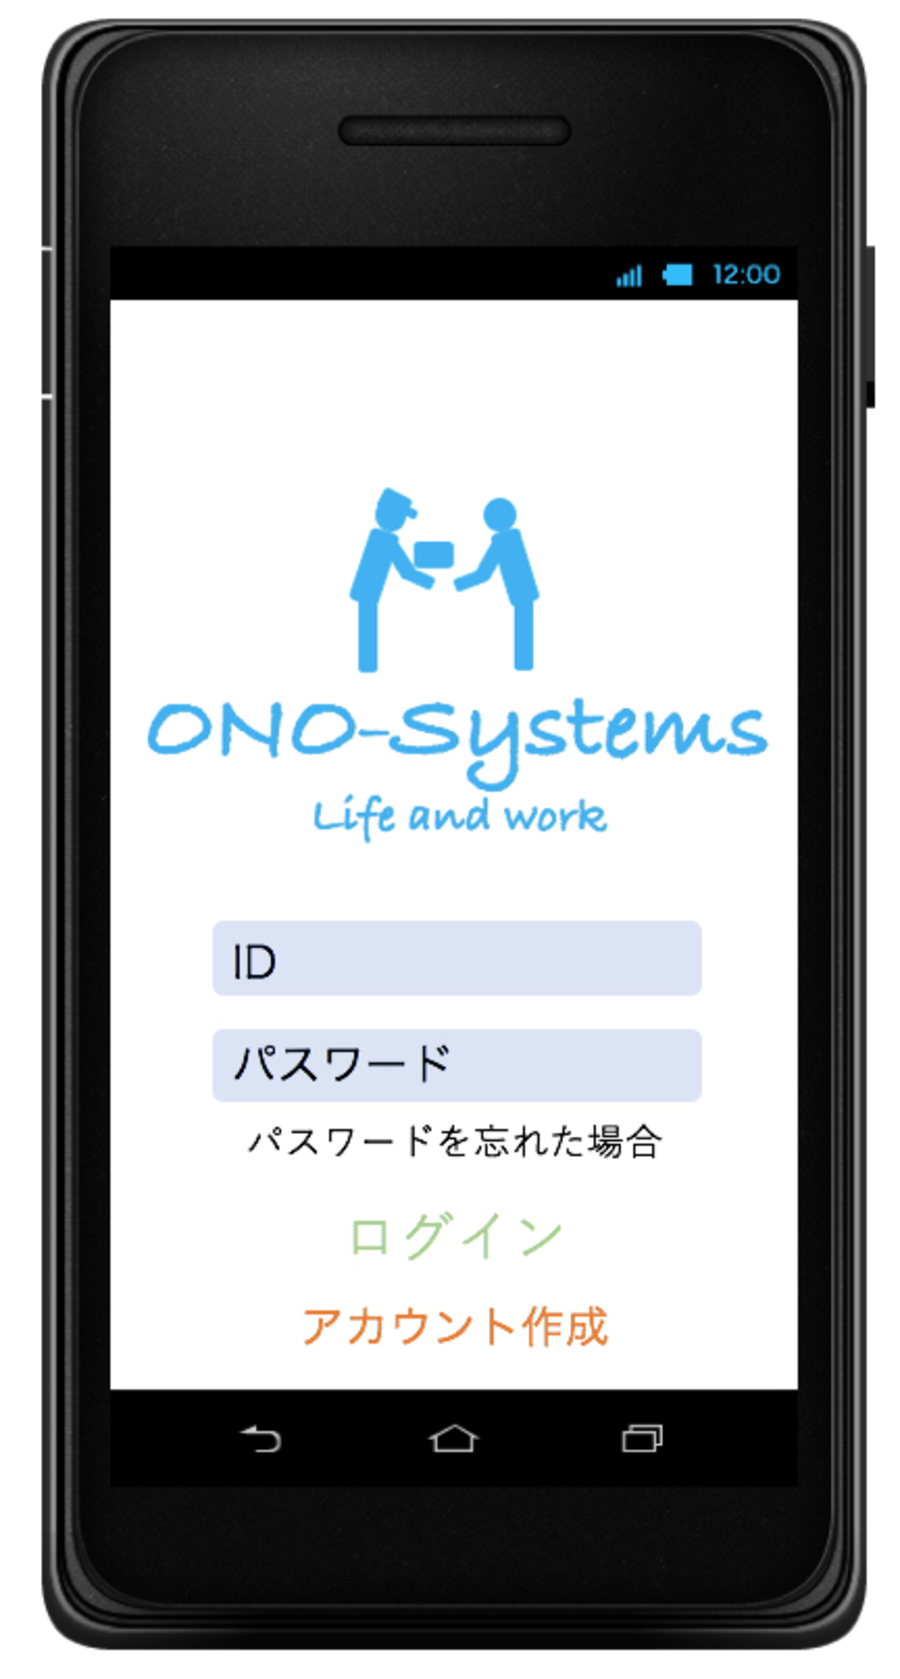
\includegraphics[width=50mm]{login}
	\caption{ログイン画面}
	\label{fig:login}
 \end{center}

\end{figure}


\subsubsection{パスワードを忘れた場合の画面}
図\ref{fig:ps_lost}は配達支援システムのパスワードを忘れた場合の画面です.この画面はホーム画面の「パスワードを忘れた場合」をタップすると表示されます.画面中央部の枠に既に登録してあるメールアドレスを入力し,送信をタップするとそのメールアドレスにパスワード再発行の為のURLが送られます.

\begin{figure}[htbp]
 \begin{center}
  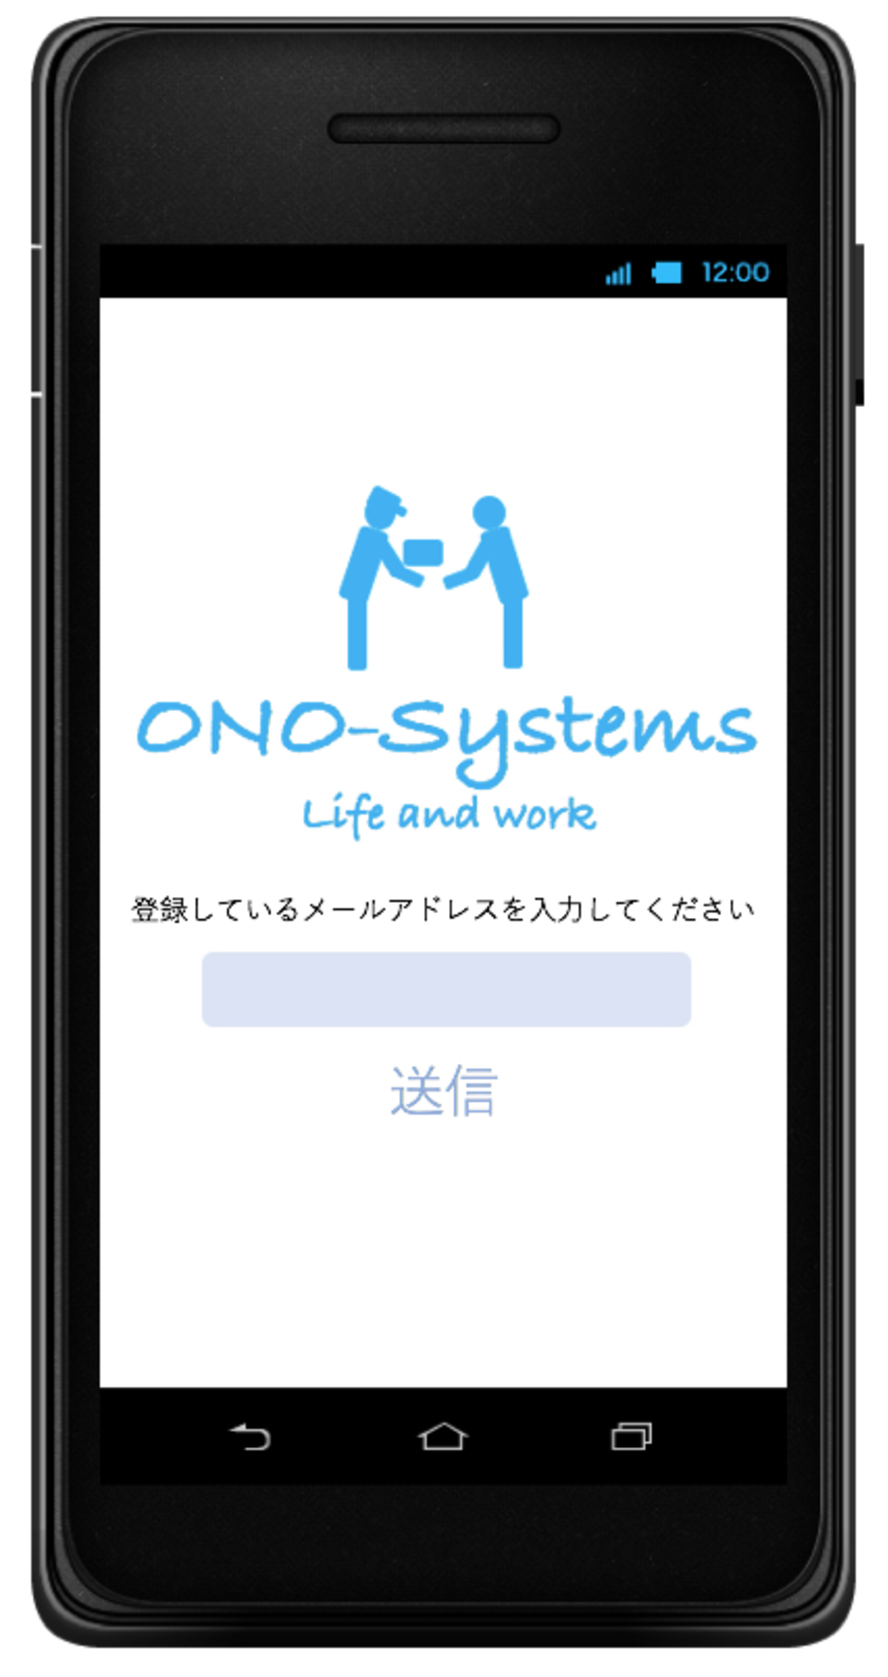
\includegraphics[width=50mm]{ps_lost}
	\caption{パスワードを忘れた場合の画面}
	\label{fig:ps_lost}
 \end{center}

\end{figure}

\subsubsection{パスワード再設定画面}
図\ref{fig:ps_change}は配達支援システムのパスワード再設定画面です.この画面は再発行の為のURLをタップすると表示されます.画面中央部の枠にパスワードを二回入力し,「パスワードの変更」をタップするとパスワード再発行が完了します.

\begin{figure}[htbp]
 \begin{center}
  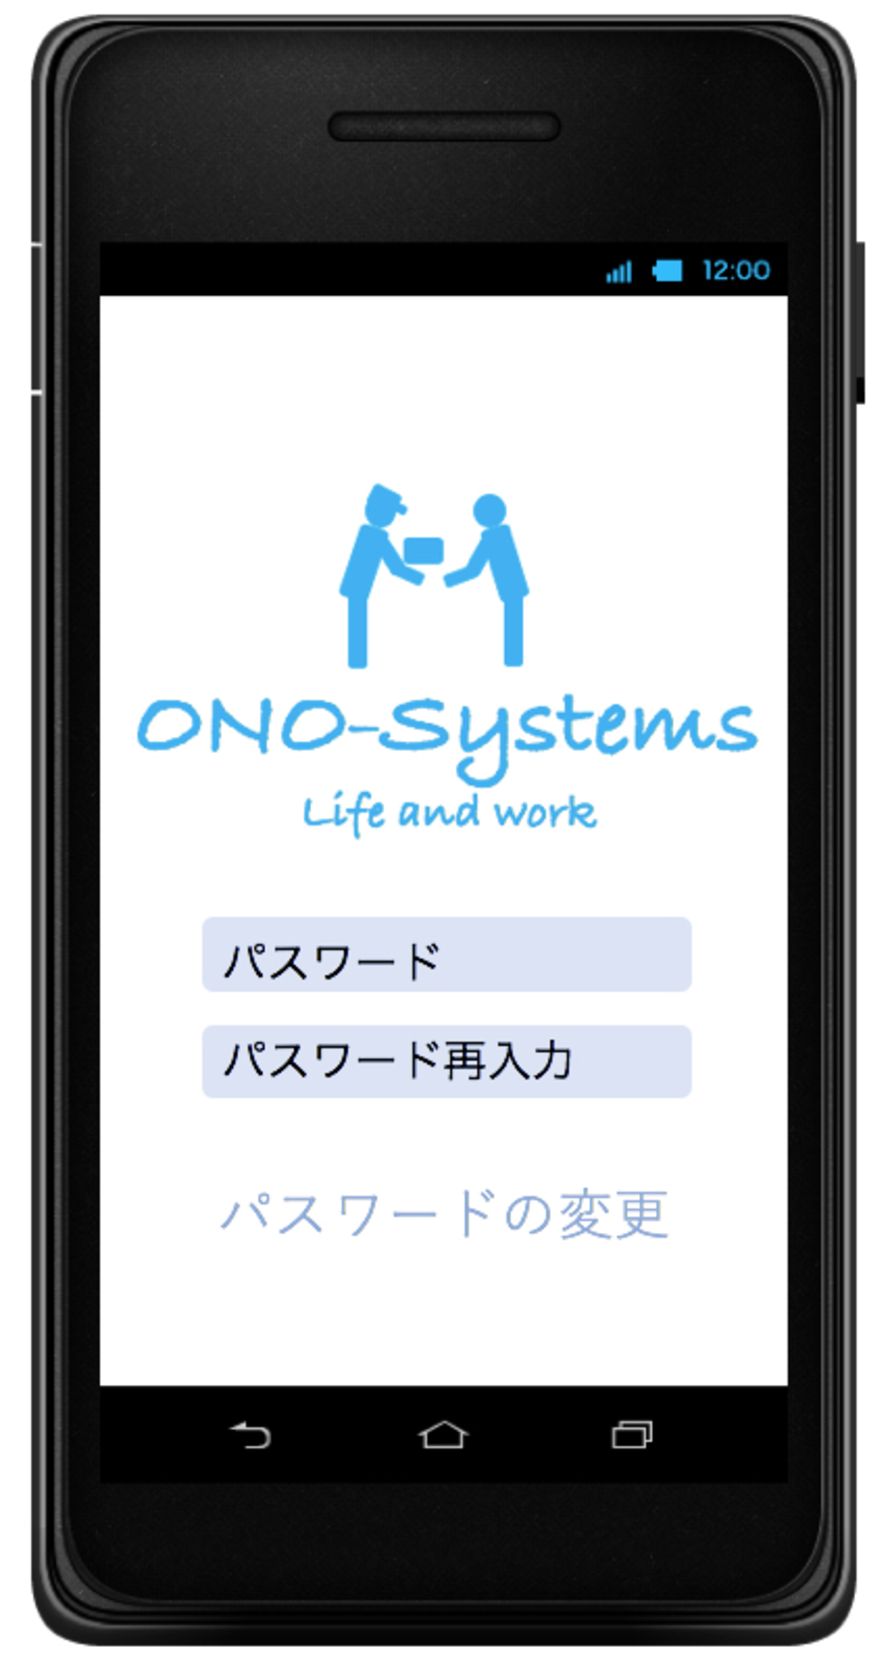
\includegraphics[width=50mm]{ps_change}
	\caption{パスワード再設定画面}
	\label{fig:ps_change}
 \end{center}

\end{figure}

\subsubsection{アカウント作成画面}
図\ref{fig:account_create}は配達支援システムのアカウント作成画面です.この画面はホーム画面の「アカウント作成」をタップすると表示されます.画面の入力欄に名前,メールアドレス,パスワード,パスワードの再入力,電話番号を入力し,「アカウント作成」をタップするとアカウントを作成することができます.アカウント作成後はユーザホーム画面に遷移します.

\begin{figure}[htbp]
 \begin{center}
  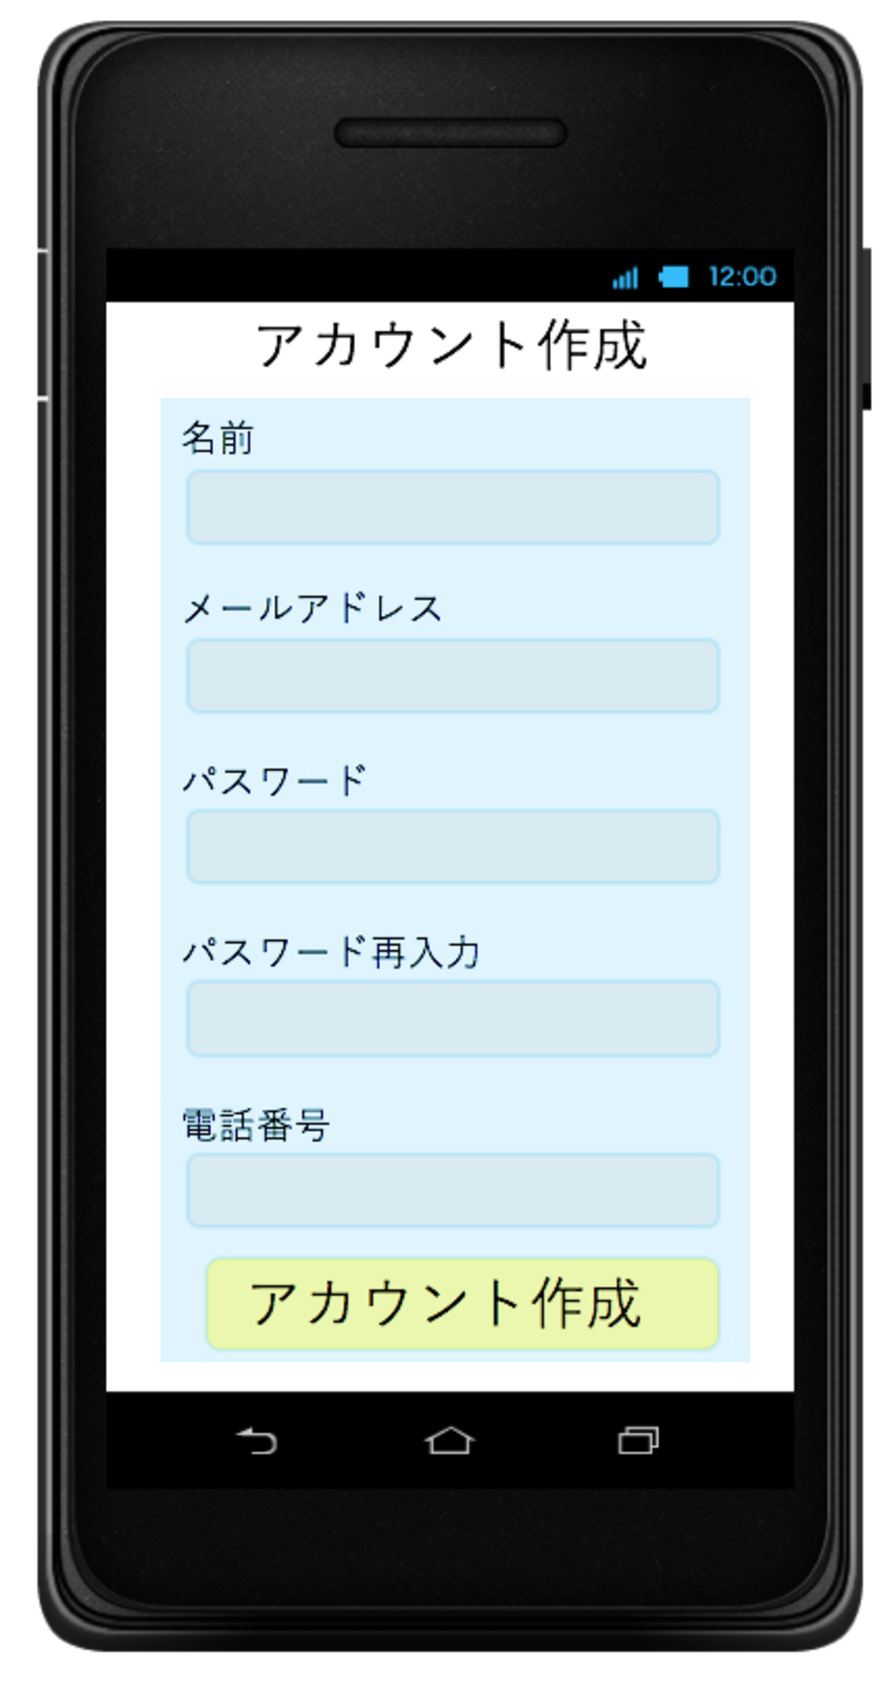
\includegraphics[width=50mm]{account_create}
	\caption{アカウント作成画面}
	\label{fig:account_create}
 \end{center}

\end{figure}



\subsubsection{ドライバーホーム画面}
図\ref{fig:driver_home}は配達支援システムのドライバーのホーム画面です.この画面はログイン画面でID,パスワードを入力し,ログインした場合に表示されます.また,既にログインしている場合はアプリ起動時に表示されます.この画面の機能は下記にて説明します.
\begin{enumerate}
	\item 利用者の選択結果のリアルタイム表示機能\\
	 \ 利用者の荷物受け取りの可否をリアルタイムに画面表示します.ドライバーが未読の間は各欄の左側に「new」と表示されます.
	\item ユーザ情報ボタン\\

	\item 距離順ソートボタン\\

	\item 時間順ソートボタン\\

	\item 配達済みソートボタン\\

	\item 受け取り可否別表示ボタン\\

	\item マップボタン\\

	\item 検索バー\\

\end{enumerate}

\begin{figure}[htbp]
 \begin{center}
  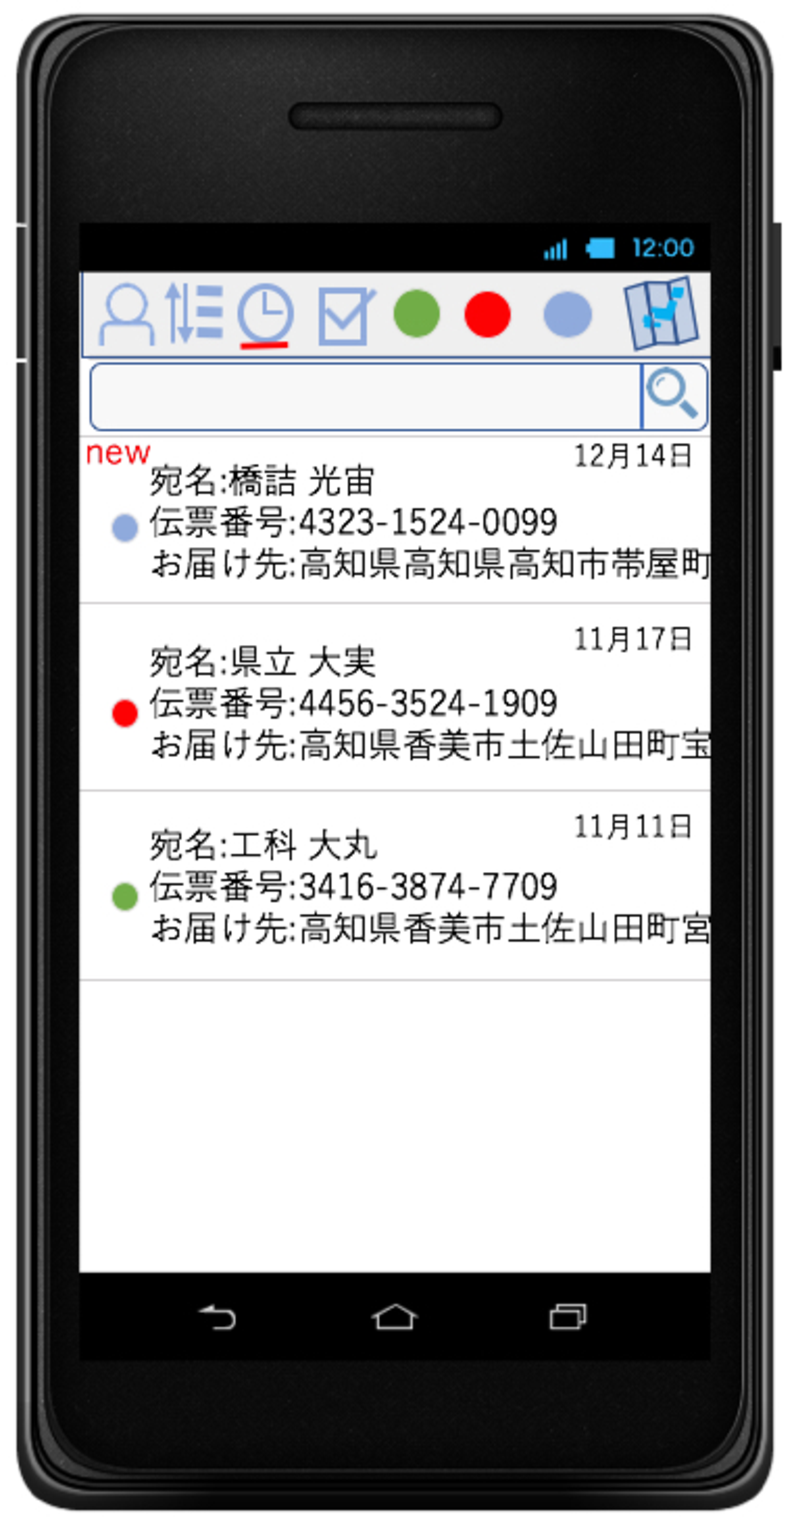
\includegraphics[width=50mm]{driver_home}
	\caption{ドライバーホーム画面}
	\label{fig:driver_home}
 \end{center}

\end{figure}




\subsubsection{ドライバーサイド画面}
図\ref{fig:driver_side}は配達支援システムのドライバーサイドの画面です.この画面はホーム画面の「ユーザ情報ボタン」をタップすると表示されます.画面の各欄にはユーザの情報(名前,メールアドレス,パスワード,パスワード再入力,電話番号)が表示されており,変更したい部分を書き換えた後に更新ボタンを押すことでユーザ情報を変更することができます.また,画面中央上部の「×」ボタンまたはバックボタンをタップするとホーム画面に遷移します.

\begin{figure}[htbp]
 \begin{center}
  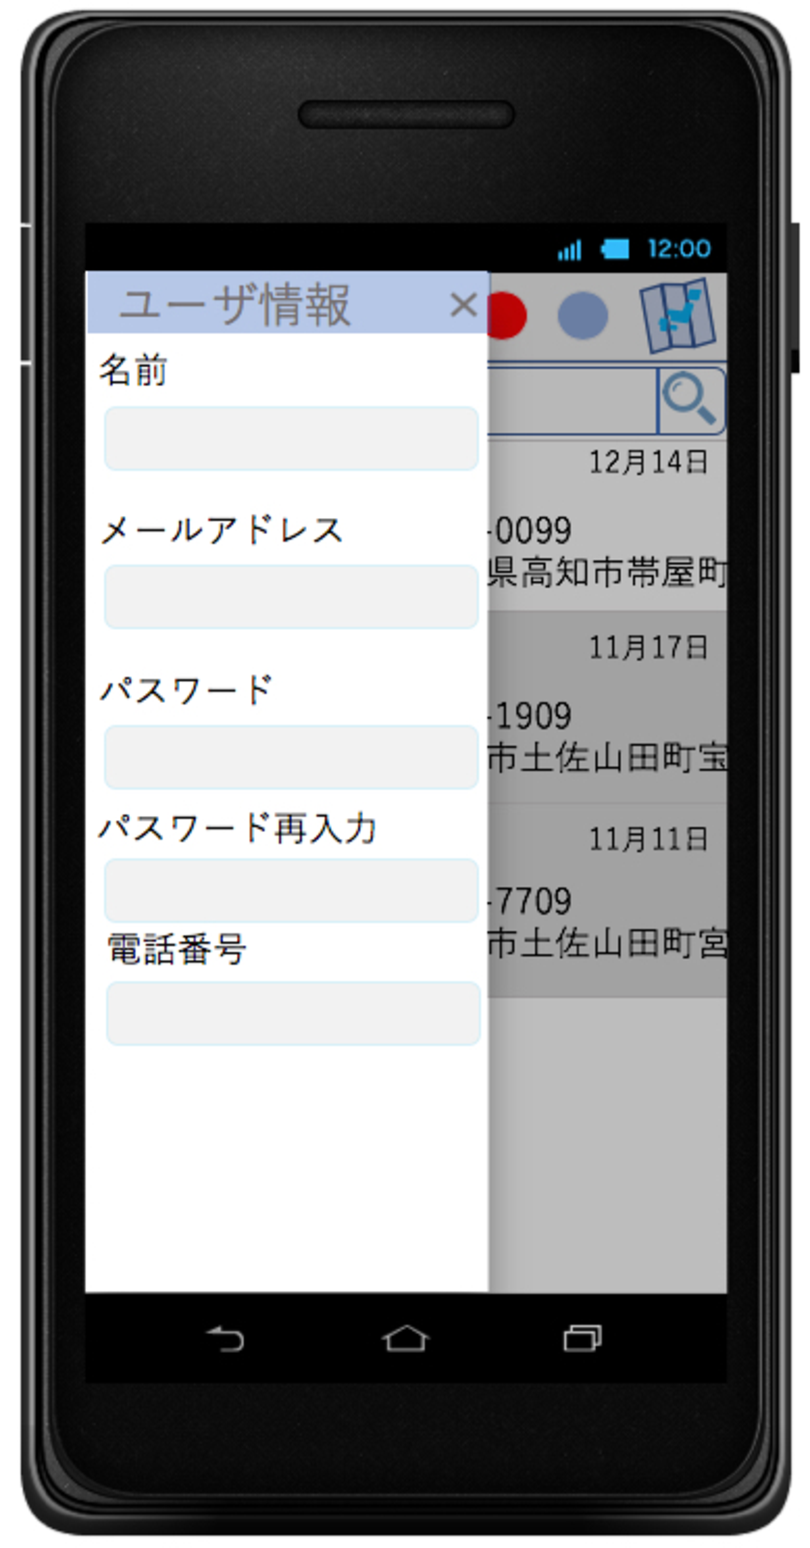
\includegraphics[width=50mm]{driver_side}
	\caption{ドライバーサイド画面}
	\label{fig:driver_side}
 \end{center}

\end{figure}

\subsubsection{ドライバー詳細画面}
図\ref{fig:driver_details}は配達支援システムのドライバー詳細画面です.この画面はホーム画面の各荷物欄をタップすると表示されます.画面には配達先の情報(宛名,伝票番号,住所,配達希望時間)が表示されており,配達希望時間の下をタップし配達希望時間を変更した後に更新ボタンをタップすると,配達希望時間を変更することができます.また,画面右上のマップボタンをタップするとマップ画面へ遷移することができ.配達完了ボタンをタップすると配達完了状態にできます.
\begin{figure}[htbp]
 \begin{center}
  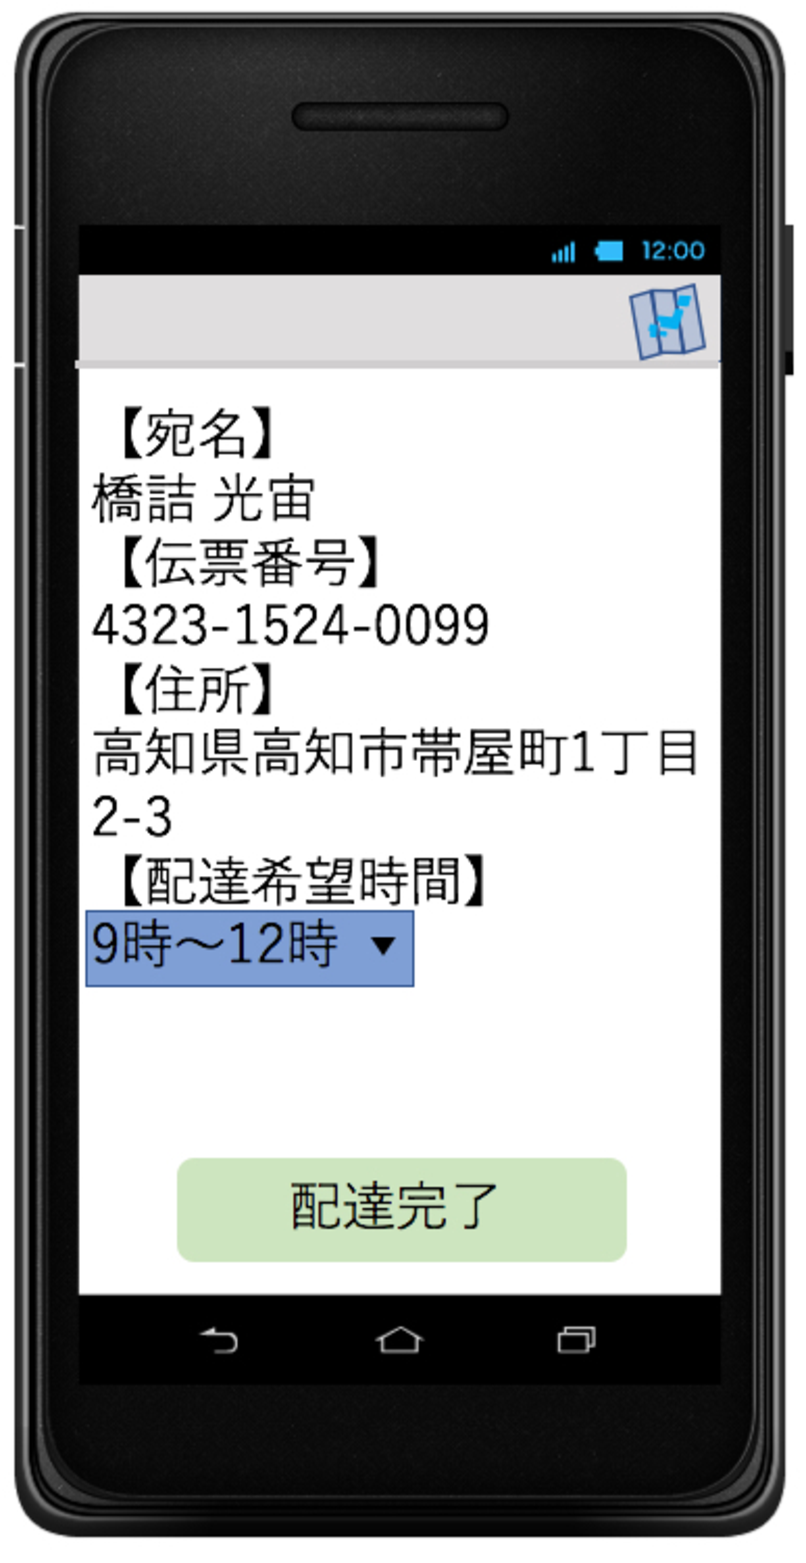
\includegraphics[width=50mm]{driver_details}
	\caption{ドライバー詳細画面}
	\label{fig:driver_details}
 \end{center}

\end{figure}




\subsubsection{マップ画面}
図\ref{fig:map}は配達支援システムのマップ画面です.この画面はホーム画面,ドライバー詳細画面のマップボタンをタップすると表示されます.この画面の機能は下記で説明します.
\begin{enumerate}
	\item 配達先表示機能\\

	\item 受け取り可否表示機能\\

	\item 絞り込み機能\\

	\item 拡大縮小機能\\

\end{enumerate}

\begin{figure}[htbp]
 \begin{center}
  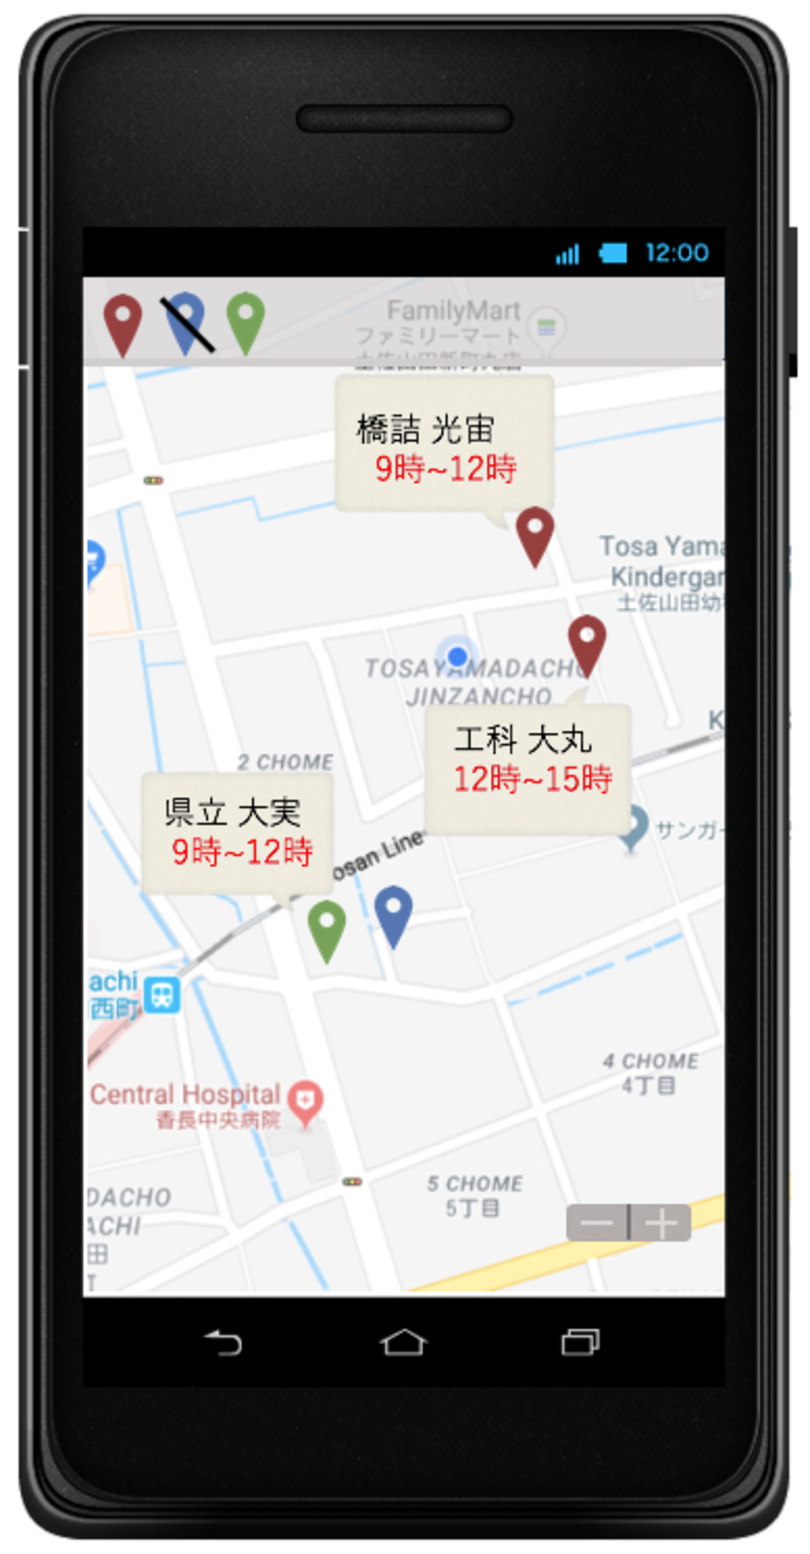
\includegraphics[width=50mm]{map}
	\caption{マップ画面}
	\label{fig:map}
 \end{center}

\end{figure}






\subsubsection{ユーザホーム画面}
図\ref{fig:user_home}は配達支援システムのドライバーのホーム画面です.この画面はログイン画面でID,パスワードを入力し,ログインした場合に表示されます.また,既にログインしている場合はアプリ起動時に表示されます.この画面の機能は下記にて説明します.
\begin{enumerate}
	\item 利用者の詳細確認機能\\

	\item ユーザ情報ボタン\\

	\item 時間順ソートボタン\\

	\item 配達済みソートボタン\\

	\item 受け取り可否別表示ボタン\\

	\item 検索バー\\

\end{enumerate}

\begin{figure}[htbp]
 \begin{center}
  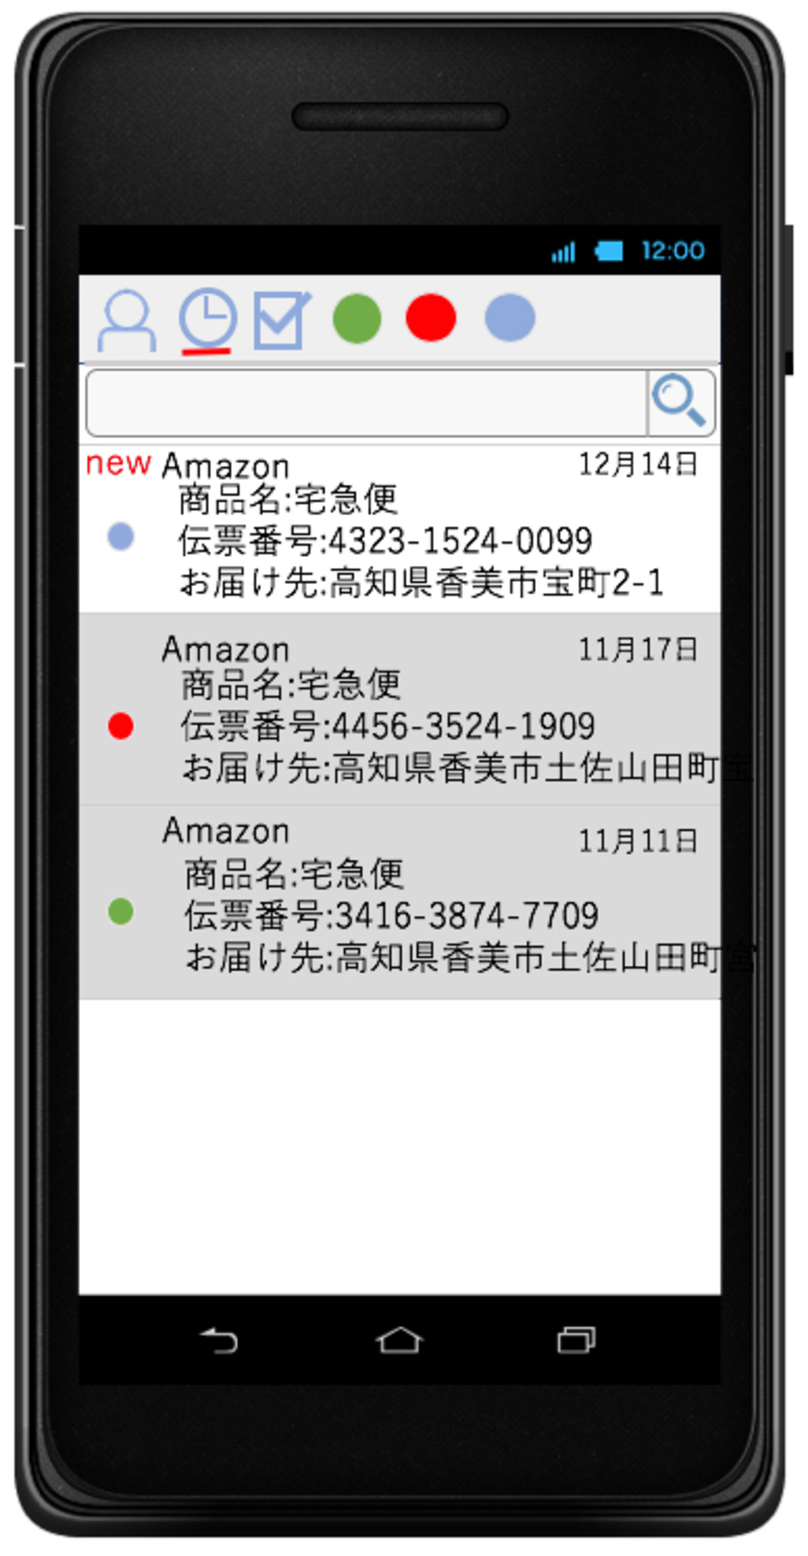
\includegraphics[width=50mm]{user_home}
	\caption{ユーザホーム画面}
	\label{fig:user_home}
 \end{center}

\end{figure}

\subsubsection{ユーザサイド画面}
図\ref{fig:user_side}は配達支援システムのユーザサイドの画面です.この画面はホーム画面の「ユーザ情報ボタン」をタップすると表示されます.画面の各欄にはユーザの情報(名前,メールアドレス,パスワード,パスワード再入力,電話番号,住所)が表示されており,変更したい部分を書き換えた後に更新ボタンを押すことでユーザ情報を変更することができます.また,画面中央上部の「×」ボタンまたはバックボタンをタップするとホーム画面に遷移します.

\begin{figure}[htbp]
 \begin{center}
  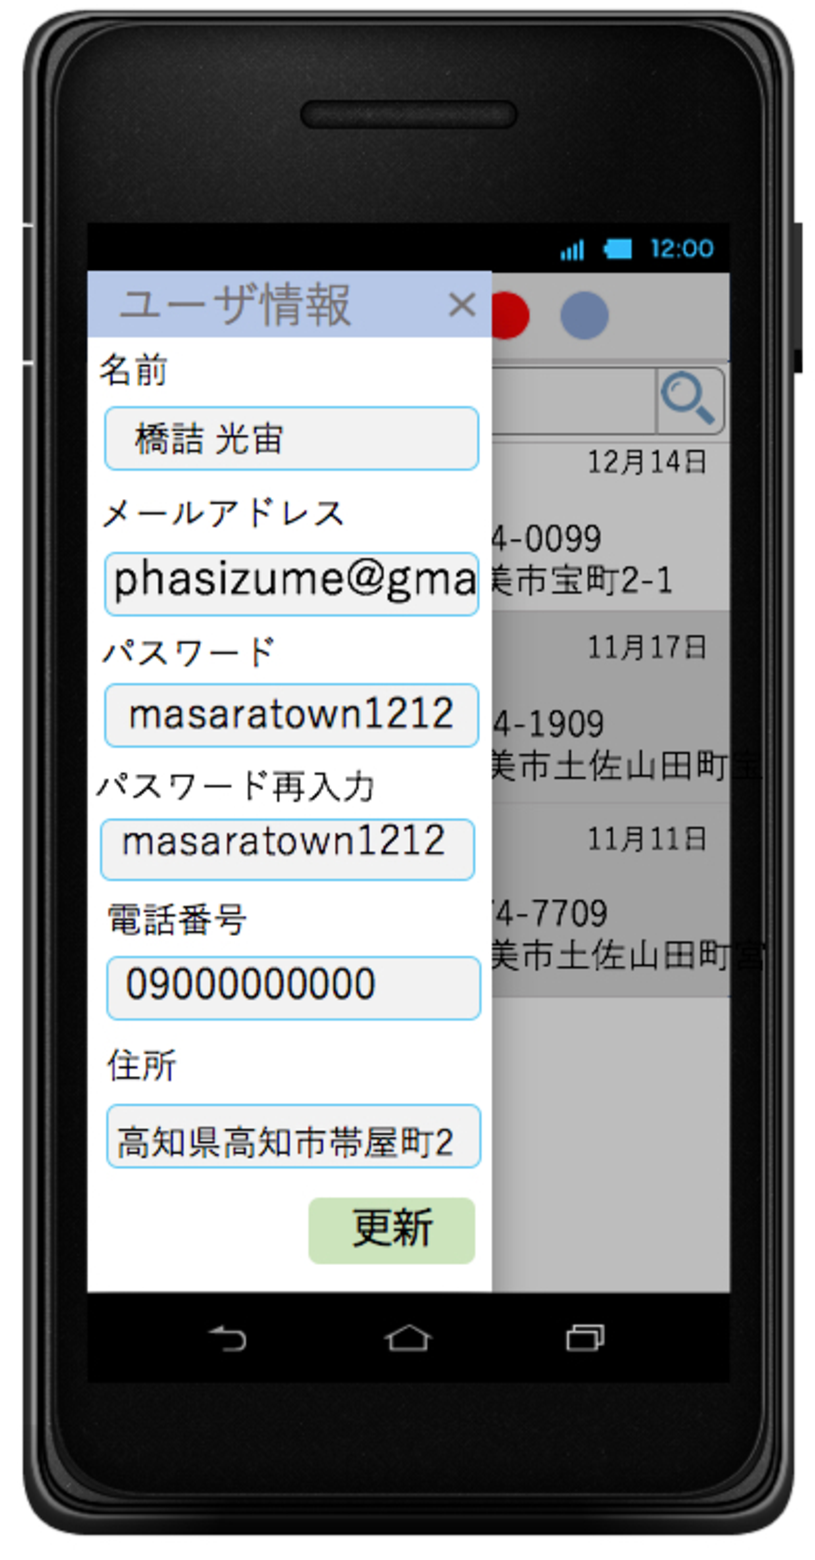
\includegraphics[width=50mm]{user_side}
	\caption{ユーザサイド画面}
	\label{fig:user_side}
 \end{center}

\end{figure}

\subsubsection{ユーザ詳細画面}
図\ref{fig:user_details}は配達支援システムのユーザ詳細画面です.この画面はホーム画面の各荷物欄をタップすると表示され,画面には商品の情報(商品名,伝票番号,お届け先,お届け日時)が表示されます.画面下の「荷物を受け取る」をタップすると配達員に荷物を受け取れると通知され,ユーザホーム画面に遷移します.また,日時変更をタップすると時間変更画面に遷移します.
\begin{figure}[htbp]
 \begin{center}
  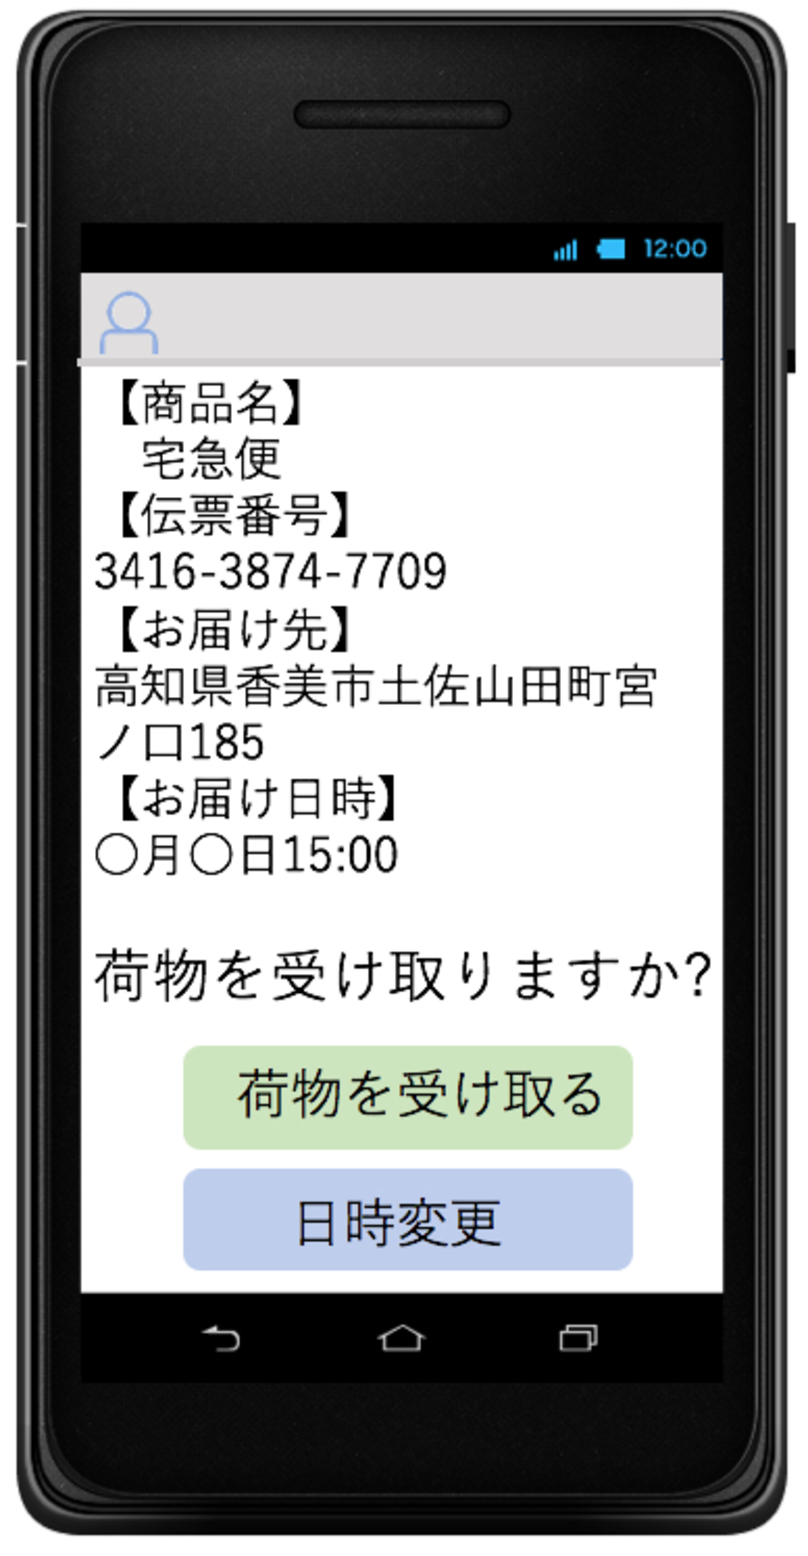
\includegraphics[width=50mm]{user_details}
	\caption{ユーザ詳細画面}
	\label{fig:user_details}
 \end{center}

\end{figure}

\subsubsection{日時変更画面}
図\ref{fig:time_change}は配達支援システムの日時変更画面です.この画面はユーザ詳細画面の「日時変更」をタップすると表示され,画面には商品の情報(商品名,伝票番号,お届け先,お届け日時)が表示されています.「○月○日15:00お届け予定」の下をタップした後に日時を変更し,「変更確定」をタップすることで配達日時を変更できます.「変更確定」タップ後はユーザホーム画面に遷移します.

\begin{figure}[htbp]
 \begin{center}
  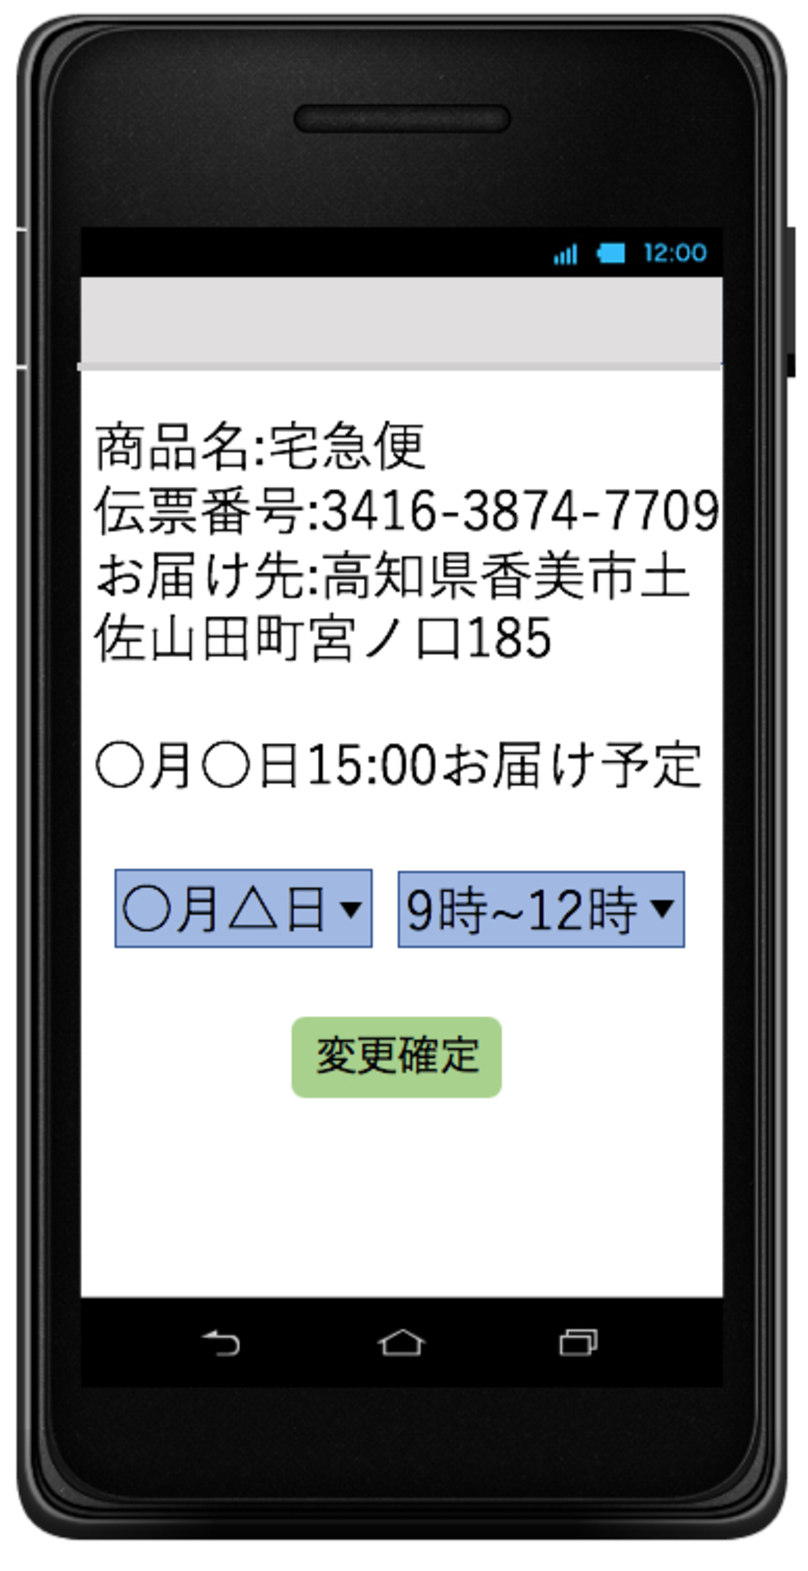
\includegraphics[width=50mm]{time_change}
	\caption{時間変更画面}
	\label{fig:time_change}
 \end{center}

\end{figure}

\section{システムのハードウェア構成}
本システムのハードウェア構成は表1の通りです.
\begin{table}[htbp]
\begin{center}
 \caption{ハードウェア構成}
  \begin{tabular}{|c|c|c|}\hline
    項目 & 数量 & 備考\\ \hline \hline
    サーバ & 1台 & AWS\\ \hline
    管理者端末 & 1台 & \\ \hline
  \end{tabular}
\end{center}
\end{table}


\section{ソフトウェア構成}
システム間のやり取りは,Java,MySQLを用いて行います.

\section{データベース設計}
本システムのデータベースには,3個のデータテーブルを用いる.各データテーブルの属性を以下に示す.

\subsection{利用者テーブル}
利用者テーブルでは,利用者に関する情報を管理する.このテーブルのデータテーブルを表2に示す.
\begin{table}[htbp]
\begin{center}
 \caption{利用者テーブル}
  \begin{tabular}{|c|c|c|c|c|c|}\hline
    属性 & データ型/長 & NULL & Key & 初期値 & その他\\ \hline \hline
    id & int(10) & NO & PRIMARY & NULL & \\ \hline
    name & varchar(64) & NO &  & NULL & \\ \hline
    address & varchar(128) & NO &  & NULL & \\ \hline
    tel & varchar(64) & NO &  & NULL & \\ \hline
    passwd & vachar(64) & NO &  & NULL & \\ \hline
  \end{tabular}
\end{center}
\end{table}

\subsection{配達者テーブル}
配達者テーブルでは,配達者に関する情報を管理する.このテーブルのデータテーブルを表3に示す.
\begin{table}[htbp]
\begin{center}
 \caption{配達者テーブル}
  \begin{tabular}{|c|c|c|c|c|c|}\hline
    属性 & データ型/長 & NULL & Key & 初期値 & その他\\ \hline \hline
    id & int(10) unsigned & NO & PRIMARY & NULL & \\ \hline
    name & varchar(64) & NO &  & NULL & \\ \hline
    store\verb|_|code & varchar(64) & NO &  & NULL & \\ \hline
    account\verb|_|type & int(1) unsigned & NO &  & NULL & \\ \hline
    passwd & vachar(64) & NO &  & NULL & \\ \hline
  \end{tabular}
\end{center}
\end{table}


\subsection{座標テーブル}
座標テーブルでは,配達者の座標に関する情報を管理する.このテーブルのデータテーブルを表4に示す.
\begin{table}[htbp]
\begin{center}
 \caption{座標テーブル}
  \begin{tabular}{|c|c|c|c|c|c|}\hline
    属性 & データ型/長 & NULL & Key & 初期値 & その他\\ \hline \hline
    id & int(10) unsigned & NO & PRIMARY & NULL & \\ \hline
    latitude & varchar(64) & NO &  & NULL & \\ \hline
    longitude & varchar(64) & NO &  & NULL & \\ \hline
		address & varchar(128) & NO &  & NULL & \\ \hline
  \end{tabular}
\end{center}
\end{table}

\section{ネットワーク構成}
本システム全体のネットワーク構成を以下の図\ref{fig:i_f}に示します.

\begin{figure}[htbp]
 \begin{center}
  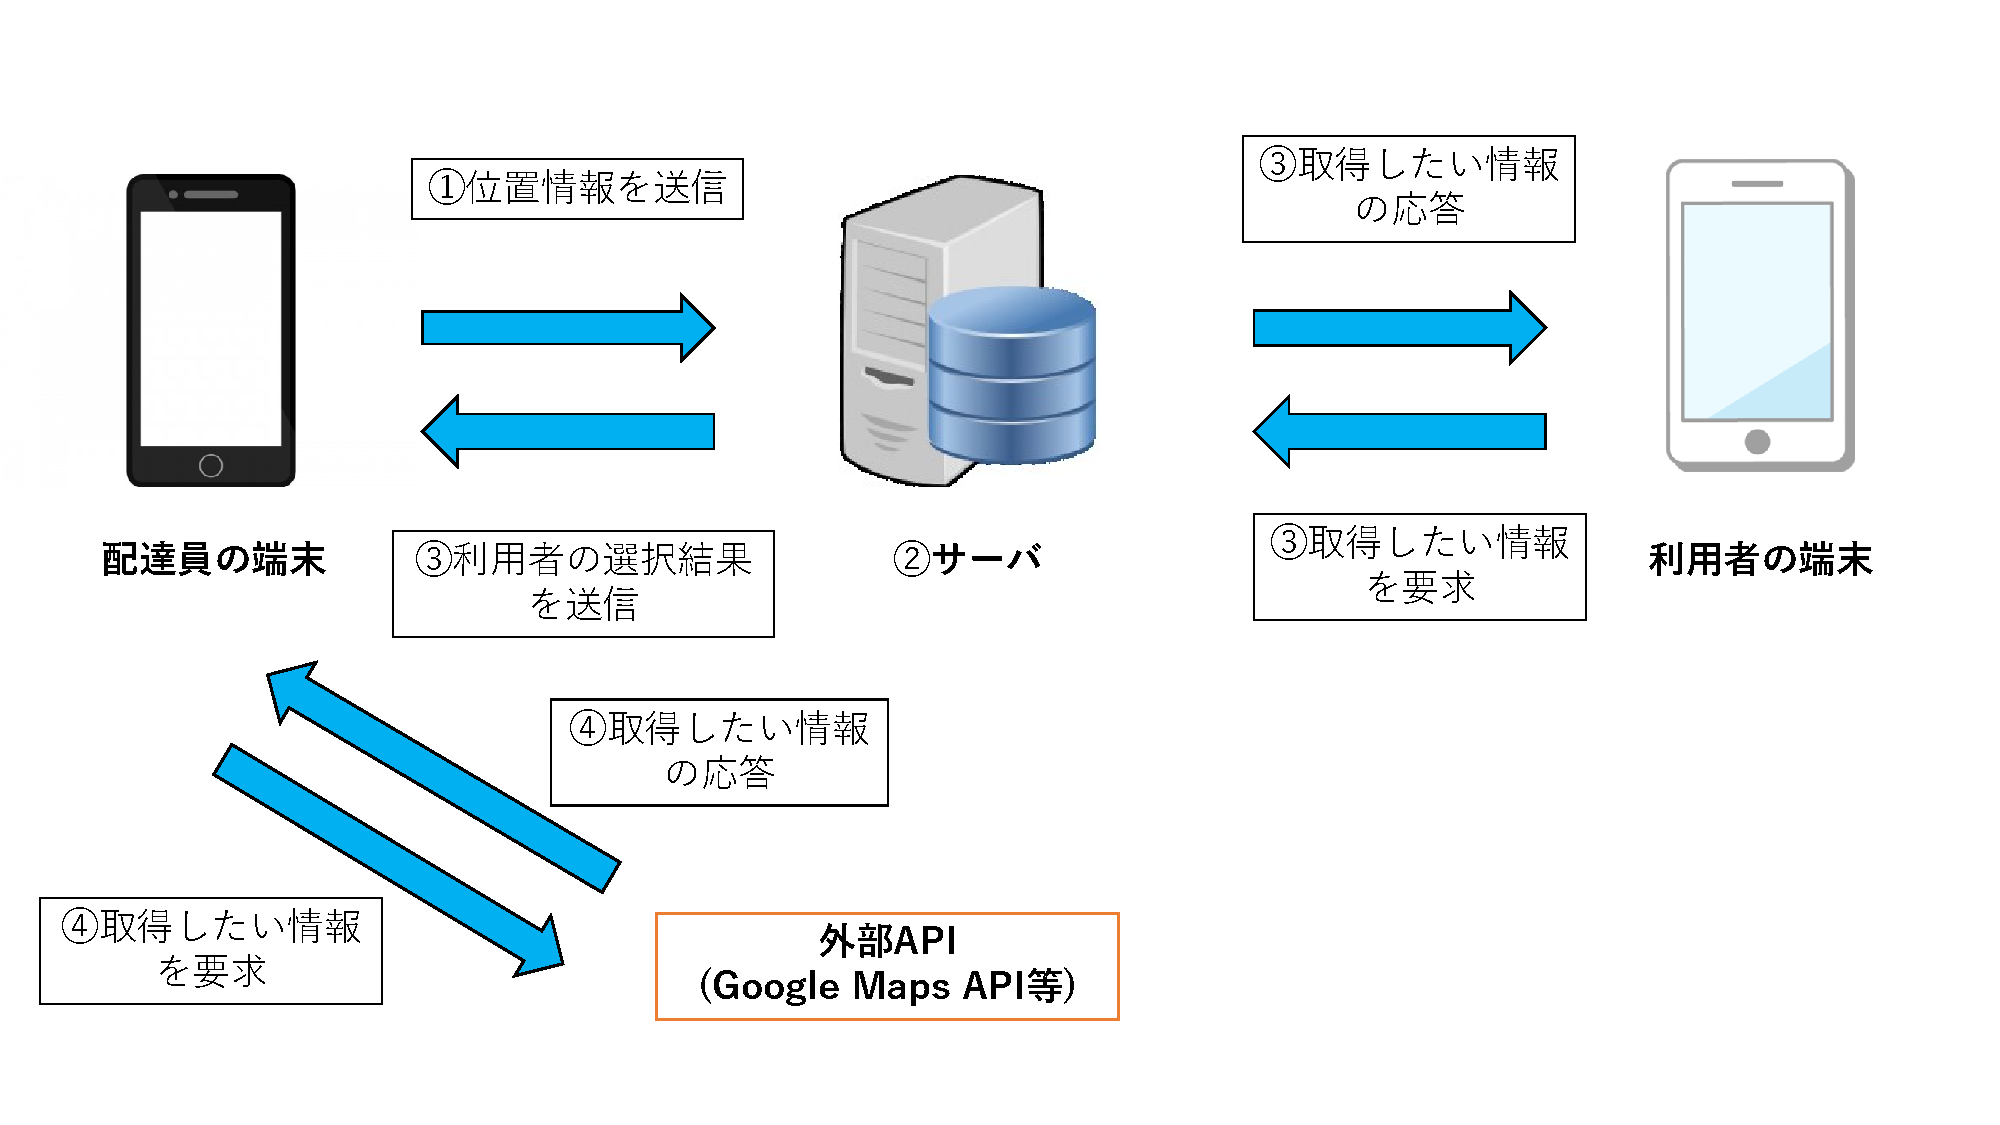
\includegraphics[width=140mm]{information_flow.pdf}
	\caption{ネットワーク構成}
	\label{fig:i_f}
 \end{center}

\end{figure}


\section{ネットワーク接続形態}
本システムでは利用者端末,管理者端末は TCP/IP を用いてサーバと通信を行います.


\section{用語の定義}
本システムでは以下のように用語を定義します.
\begin{itemize}
 \item 利用者:ネットショッピングなどを通じて商品を購入して,自宅に配送するように指定した消費者
 \item 配達員:宅配業者の従業員で商品をお客様の家まで届ける人
\end{itemize}

\begin{thebibliography}{9}

\bibitem{ref1}
国土交通省,
\newblock ``宅配便の再配達削減に向けて'',\\
\newblock \url{http://www.mlit.go.jp/seisakutokatsu/freight/re_delivery_reduce.html}, \\
2018/10/11
\bibitem{ref2}
エン・ジャパン株式会社,
\newblock ``ヤマト運輸株式会社 中部支社のドライバー ★平均月収35万円。無理なく年収400万円が見込めます。'',\\
\newblock \url{https://employment.en-japan.com/desc_770664/}, \\
2018/10/11
\end{thebibliography}

\end{document}
